

\documentclass[letterpaper,12pt]{article}
\usepackage{tabularx} % extra features for tabular environment
\usepackage{amsmath}  % improve math presentation
\usepackage{float}
\usepackage{pdfpages}

\usepackage{multicol}
\usepackage{graphicx} % takes care of graphic including machinery
\graphicspath{ {./figures/} }
%\usepackage[margin=1in,letterpaper]{geometry} % decreases margins
%\usepackage{cite} % takes care of citations
\usepackage[final]{hyperref} % adds hyper links inside the generated pdf file
\hypersetup{
    colorlinks=true,       % false: boxed links; true: colored links
    linkcolor=blue,        % color of internal links
    citecolor=blue,        % color of links to bibliography
    filecolor=magenta,     % color of file links
    urlcolor =blue         
}
\usepackage[margin = 1in,headsep=0.5cm,headheight=2cm,letterpaper]{geometry} 

\usepackage{fancyhdr}
\pagestyle{fancy}
\lhead{Student 1 : Ahmet Akman 2442366 \\ Student 2: Yusuf Toprak Yıldıran 2444149 \\ Assistant: Onur Selim Kılıç}
\rhead{Date: \today \\ Group: Wednesday Morning - 5} 
%\cfoot{center of the footer!}
\renewcommand{\headrulewidth}{0.1pt}



\begin{document}
\thispagestyle{empty}

\title{Spring 2022 EE214 Experiment 7  \protect\\ Active RC Filters}
\author{Ahmet Akman 2442366 \protect\\ Yusuf Toprak Yıldıran 2444149 \protect\\ Assistant: Onur Selim Kılıç}
\date{\today}
\maketitle
\tableofcontents
%\begin{abstract}
%abstract
%\end{abstract}
\section{Introduction}
In this experiment, active RC low-pass and band-pass filters will be studied. Their cut-off and center frequencies will be found manually and using the BenchVue test flow program, and frequency and phase responses will be plotted. Afterward, the passband bandwidth of the band-pass filter will be measured, and by making some adjustments to the band-pass filter circuit, its bandwidth will be increased.


\section{Experimental Results and Discussion}
The results of the experiment are discussed in the following steps.
\subsection{Step 1}

In this part, the circuit in figure 1 is set with an input sine wave of 1V peak. Then, the max output voltage is found and recorded as the center frequency by manually changing the frequency. Afterward, half-power frequency, which is equal to 0.7 times the center frequency, is found by trying the frequencies, and these values are recorded in table 1.   
\begin{figure}[H]
    \centering
    \includegraphics[width = 0.75\textwidth]{{lowpass.png}}
    \caption{circuit for step 1}
\end{figure}


\begin{table}[H]
    \begin{center}
        \caption{Measurements}
        \vspace{2mm}
        \begin{tabular}{|| c | c | c||} 
            \hline
              \(\omega_c\) & \(|H(w_c)|\) & \(arg(H(w_c))\)   \\ [0.5ex] 
            \hline\hline
              1570Hz & 3.29V & 107\(\circ \) \\ 
             \hline \hline \hline
              \(\omega_o\) & \(|H(w_o)|\) &  arg(\(H(w_o)\))   \\ [0.5ex] 
            \hline\hline
              900 Hz & 4.7V & 50\( \circ \) \\ 
            \hline
        \end{tabular}
    \end{center}
\end{table}

Afterward, frequency and phase response of the cicuit are obtained using computer BenchVue test flow with DC sweep from \(\frac{f_c}{5}\) to \(5f_c\) with the steps \(\frac{f_c}{10}\).

After making necessary test flow settings and running the test, magnitude and frequency responses of the circuit are obtained. Then, data are exported to MATLAB, and \(w_0\),\(w_1\), and \(w_2\) are determined from the magnitude response plot and shown in Figure 2.  

\begin{figure}[H]
    \centering
    \includegraphics[width = 1 \textwidth]{{1_1.png}}
    \caption{Magnitude and Phase response of circuit 1}
\end{figure}

\subsection{Step 2}
In this step the band pass circuit given in Figure 3 is constructed.
\begin{figure}[H]
    \centering
    \includegraphics[width = 0.75\textwidth]{{bandpass.png}}
    \caption{Circuit for step 2}
\end{figure}

\subsubsection{a)}
The frequency magnitude and frequency phase response of the circuit is obtained and given in Figure 4.

\begin{figure}[H]
    \centering
    \includegraphics[width = 1\textwidth]{{2_1.png}}
    \caption{Magnitude and Phase response of circuit 2}
\end{figure}

So the half-power frequency, center frequency values, and the passband bandwidth is determined and given in Table 2.

\begin{table}[H]
    \begin{center}
        \caption{Measurements}
        \vspace{2mm}
        \begin{tabular}{|| c | c | c | c ||} 
            \hline
              \(\omega_o\) & \( \omega_{c1} \) & \(\omega_{c2}\)  & \(\Delta \omega\) \\ [0.5ex] 
            \hline\hline
              20.350 kHz & 11.850 kHz & 43.380kHz & 31.530 kHz  \\ 
             \hline 
        \end{tabular}
    \end{center}
\end{table}
It can be said that different from passive band-pass filters, active filters also have a positive gain value. This means the specified frequencies also can be amplified with an active filter. Also, it  can be said that experimental results are also consistent with the results obtained in the simulations.
\subsubsection{b)}
The resistors on the positive feedback side, a.k.a. the resistors of 6.8k and 10k, are disconnected, and the V+ terminal is grounded. As a result, the frequency magnitude and frequency phase responses are obtained and shown in Figure 5.


\begin{figure}[H]
    \centering
    \includegraphics[width = 1 \textwidth]{{2_2.png}}
    \caption{Magnitude and Phase response of circuit 2 without the resistors}
\end{figure}
So the half-power frequency, center frequency values, and the passband bandwidth is determined and given in Table 3.

\begin{table}[H]
    \begin{center}
        \caption{Measurements}
        \vspace{2mm}
        \begin{tabular}{|| c | c | c | c ||} 
            \hline
              \(\omega_o\) & \( \omega_{c1} \) & \(\omega_{c2}\)  & \(\Delta \omega\) \\ [0.5ex] 
            \hline\hline
              24.100 kHz & 11.300 kHz & 49.650kHz & 38.350 kHz  \\ 
             \hline 
        \end{tabular}
    \end{center}
\end{table}
So it can be said that even though the first half-power frequency is quite close to the first high-q setup, the second half-power frequency is different. It can be concluded that the resistors that provide feedback to the non-inverting terminal of the op-amp determine where the low pass limit takes place.  Also, it  can be said that experimental results are also consistent with the results obtained in the simulations.

\section{Conclusion}
In this experiment, active RC low-pass and band-pass filters are studied. Their cut-off and center frequencies are found manually and using the BenchVue test flow program, and frequency and phase responses are plotted. Afterward, the passband bandwidth of the band-pass filter is measured, and by making some adjustments to the band-pass filter circuit, its bandwidth is increased.

\section*{Appendix A}
\begin{itemize}
    \item PreLab Preparation 2 hours
    \item Experimental Work 2  hours
    \item Report Writing 9 hours
\end{itemize}

\end{document}

%%%%%%%%%%%%%%%%%%%%%%   EXAMPLE TABLE   %%%%%%%%%%%%%%%%%%%%%%%%%%%%%%%%
\begin{table}[H]
\begin{center}
    \caption{Resistance reading by color code convention.}
    \vspace{2mm}
    \begin{tabular}{||c | c | c||} 
        \hline
        Color Order & Value & Tolerance \\ [0.5ex] 
        \hline\hline
        Brown / Black / Red / Gold & 1k\( \Omega \) & \( \% \) 5  \\ 
        \hline
        Yellow / Violet / Red / Gold & 4.7k\( \Omega \) & \( \% \) 5   \\
        \hline
        Brown / Grey / Orange / Gold & 18k\( \Omega \) & \( \% \) 5  \\ [1ex] 
        \hline
    \end{tabular}
\end{center}
\end{table}


%%%%%%%%%%%%%%%%%%%%%%   EXAMPLE IMAGE   %%%%%%%%%%%%%%%%%%%%%%%%%%%%%%%%
\begin{figure}[H]
\centering
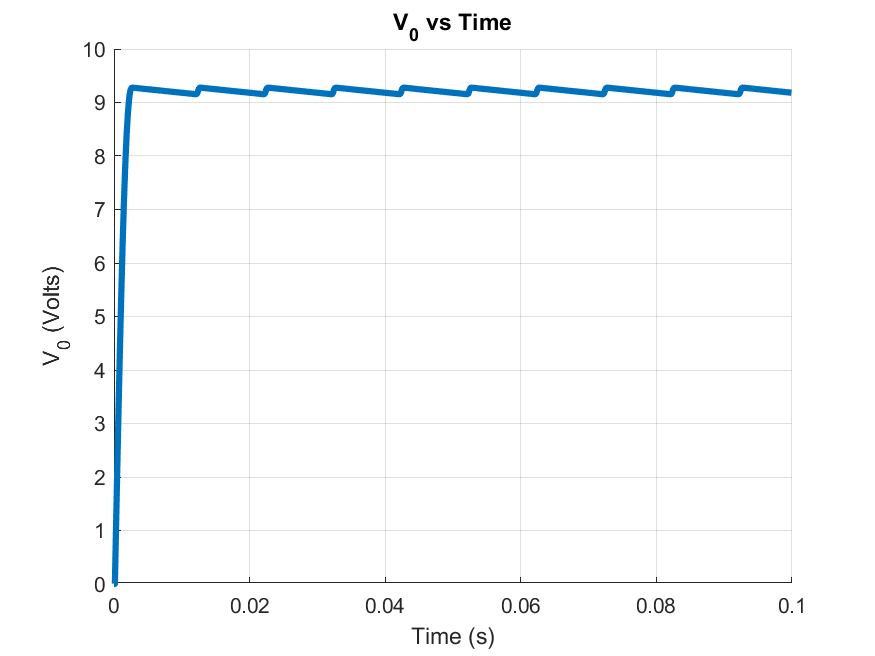
\includegraphics[width = 0.75\textwidth]{5.png}
\caption{Circuit schematic for the step 5}
\end{figure} 

%%%%%%%%%%%%%%%%%%%%%%   EXAMPLE IMAGE FROM PDF   %%%%%%%%%%%%%%%%%%%%%%%%%%%%%%%%
\begin{figure}[H] \centering{
    \includegraphics[scale=0.25]{2a_plot.pdf}}
    \caption{Experiment 2}
\end{figure}


